\chapter{PENDAHULUAN}\label{pendahuluan}
\section{Latar Belakang}\label{latar belakang}

Indonesia merupakan pengguna energi terbesar di Asia Tenggara, yaitu lebih dari 36\% penggunaan energi primer Asia Tenggara. Antara tahun 2000 dan 2015, produk domestik bruto (PDB) Indonesia bertambah dua kali lipat dan kebutuhan listrik meningkat 150\%. Pertumbuhan ekonomi mendorong kebutuhan energi Indonesia. Pengguna energi terbesar Indonesia tahun
2015 adalah sektor rumah tangga (38\%) dan industri dan jasa (29\%), diikuti oleh transportasi (27\%) (Gambar\ref{fig:1:energy}).
\begin{figure}[!h]
	\centering
	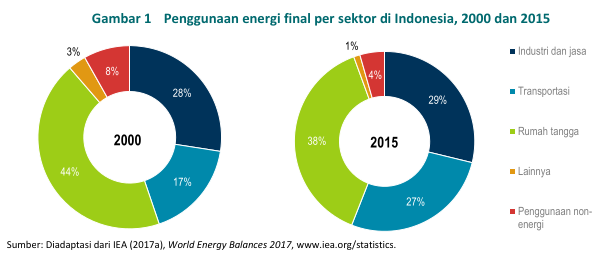
\includegraphics[width=1\textwidth]{figures/EnergyUsage}
	\caption{Penggunaan energi final per sektor di Indonesia, 2000 dan 2015}
	\label{fig:1:energy}
\end{figure}
Efisiensi sangat penting dilakukan untuk menghemat energi. Penggunaan teknologi pendingin ruangan yang lebih efisien diperkirakan mampu
menghemat tagihan pelanggan listrik USD 690 juta per tahun di tahun 2030. Kebutuhan
pendingin ruangan tumbuh cepat dan diperkirakan bertambah dua kali lipat antara tahun
2016 dan 2020 \cite{IEA}.

Ruangan pada setiap bangunan umumnya menggunakan pendingin ruangan (AC) untuk mencapai kondisi yang nyaman bagi penghuni di dalamnya. Padahal hal tersebut kurang tepat. Sesungguhnya, penghuni tidak menginginkan kondisi ruang yang lebih dingin ataupun lebih panas dari keadaan awalnya. Penghuni ruang menginginkan kondisi ruangan yang nyaman bagi tubuh mereka. Kondisi ini yang disebut sebagai kenyamanan termal. Kenyamanan termal yang dimaksud tidaklah sesederhana upaya untuk menurunkan suhu di suatu ruangan. Kenyaman termal bergantung juga kepada sensasi termal tubuh manusia. Sehingga, kebutuhan energi dalam pemenuhan kenyamaan termal tersebut dapat dikatakan cukup tinggi.

Kenyamanan termal penting untuk kesehatan dan kebugaran tubuh manusia. Hal tersebut berpengaruh terhadap produktivitas manusia dalam melakukan kegiatan. Kurangnya kenyamanan termal dapat mengakibatkan kondisi stres bagi penghuni bangunan. Apabila kondisi bangungan terlalu panas, maka penghuni akan merasa lelah. Apabila kondisi bangunan terlalu dingin, maka penghuni akan merasa gelisah dan bimbang.

Kenyamanan termal secara fisiologis bergantung kepada proses perpindahan kalor antara tubuh dan lingkungan dimana respon fisiologis tubuh berupaya untuk mempertahankan suhu inti tubuh agar tetap bernilai konstan. Untuk mempelajari respon fisiologis tersebut, dibutuhkan sebuah \textit{climate chamber} dimana kondisi iklim di dalamnya dapat dikendalikan sesuai dengan kebutuhan penelitian.

\textit{Climate chamber} merupakan suatu ruangan tertutup yang digunakan untuk menguji efek dari kondisi lingkungan yang ditentukan pada objek biologis, produk industri, bahan, dan/atau perangkat elektronik. Pada penulisan ini, \textit{climate chamber} yang dimaksud berfokus pada objek biologis mengenai penelitian kenyamanan termal. Dalam melakukan penelitian kenyamanan termal, peneliti tersebut membutuhkan suatu \textit{climate chamber} untuk dapat melakukan pengujian. Kondisi lingkungan termal di dalam \textit{climate chamber} dapat berubah sesuai dengan skema pengujian. Terdapat 6 faktor lingkungan termal yang mempengaruhi kenyamanan termal. Faktor lingkungan termal tersebut meliputi tingkat metabolisme tubuh, insulasi pakaian, suhu udara, suhu radian, kecepatan udara dan kelembapan \cite{ASHRAE55}.

\textit{Climate chamber} dapat terwujud jika kondisi iklim di dalamnya dapat dikendalikan sesuai dengan kebutuhan penelitian. Maka dari itu, dibutuhkan suatu sistem kendali yang mampu mengendalikan lingkungan termal pada \textit{climate chamber}. \textit{Climate chamber} memiliki banyak nilai masukan dan keluaran atau dikatakan sebagai sistem MIMO (\textit{multiple input multiple output}). Untuk dapat mengendalikan sistem MIMO, diperlukan sistem kendali cerdas (\textit{intelligent control system}). Salah satu sistem kendali cerdas yang dapat digunakan untuk sistem MIMO ini yaitu pengendali dengan menggunakan jaringan saraf tiruan (\textit{neural network controller}).

%Penulis mengambil studi kasus pada \textit{climate chamber} di Departemen Teknik Nuklir dan Teknik Fisika (DTNTF) UGM yang digunakan sebagai ruang uji penelitian kenyamanan termal. \textit{Climate chamber} DTNTF dilengkapi dengan beberapa perangkat sensor untuk mengukur faktor lingkungan termal. Sensor yang digunakan yakni sensor suhu, sensor kelembaban relatif dan sensor kecepatan udara. \textit{Climate chamber} DTNTF pun dilengkapi dengan perangkat aktuator berupa \textit{Air Conditioner} (AC) dan \textit{heater} sebagai sistem \textit{Heating, Ventilation, and Air Conditioning} (HVAC). Didalamnya pun tersedia perangkat komputer yang digunakan sebagai \textit{computer server} untuk basis data (\textit{database}) pengukuran sensor parameter lingkungan termal. Selain itu, perangkat komputer digunakan pula untuk proses pengisian kuesioner dalam penelitian kenyamanan termal. Semua sistem yang digunakan pada \textit{climate chamber} ini masih dioperasikan secara manual.

%Untuk mengkondisikan lingkungan termal, digunakan perangkat \textit{Air Conditioner} (AC) dan \textit{heater} sebagai \textit{manipulator} lingkungan. Agar perangkat AC dan \textit{heater} dapat bekerja secara optimal maka diperlukan suatu sistem pengendalian yang mampu mengendalikan lingkungan termal sesuai dengan tuntutan perancangan. \textit{Climate Chamber} membutuhkan suatu sistem kendali yang mampu mengatur dan menjaga nilai suhu dan kelembapan udara di dalamnya. Sistem kendali lingkungan termal untuk ruang uji termal terdiri dari 3 komponen berupa sensor, pengendali, dan aktuator. Hal ini menjadikan komponen pengendali sebagai salah satu komponen penting dalam menciptakan \textit{climate chamber} yang terkendali.

%Dalam melakukan perancangan sistem kendali, proses perancangan terbagi menjadi 2 langkah, yakni proses identifikasi sistem dan proses perancangan pengendali. Dalam proses identifikasi sistem, peneliti pada umumnya merujuk kepada pemodelan \textit{plant}. Pada penulisan ini, penulis berfokus pada proses perancangan pengendali menggunakan jaringan saraf tiruan. Pemodelan \textit{plant} didapatkan dari penelitian sebelumnya yang menggunakan aplikasi piranti lunak IES-VE\cite{skripsi1}.

%Pengendali dari sistem kendali lingkungan termal pada ruang uji termal dapat dibangun dengan berbagai sistem kendali. Salah satu sistem kendali yang cukup populer adalah sistem kendali cerdas (\textit{Intelligent Control System}). Pada sistem kendali cerdas, kecerdasan buatan diterapkan pada algoritma kendali yang kemudian ditanamkan pada pengendali sehingga mampu membangun suatu pengendali yang dapat bekerja dengan adaptif terhadap kondisi yang berubah-ubah. Cabang kecerdasan buatan yang kerap digunakan pada sistem ini yaitu \textit{Machine Learning}. \textit{Machine Learning} bekerja dengan mengolah data-data yang diberikan berupa pasangan nilai masukan dengan nilai keluaran. Kemudian program komputer ini akan belajar dari data-data tersebut melalui metode yang dipilih. Salah satu metode yang dapat digunakan untuk sistem kendali lingkungan termal adalah metode jaringan saraf tiruan (\textit{Artificial Neural Network}).

%Jaringan saraf tiruan pada penulisan ini memiliki tugas untuk menjaga nilai suhu dan kelembapan udara pada ruang uji termal \textit{climate chamber} agar bernilai tetap sesuai dengan tuntutan perancangan yang ditentukan oleh penulis. Sehingga ruang uji termal kelak dapat dipandang sebagai lingkungan termal yang terkendali dan dapat digunakan untuk menguji respon fisiologis tubuh manusia terkait kenyaman termal yang dirasakan oleh penghuni ruang.

\section{Perumusan Masalah}
Penulis mengambil studi kasus pada \textit{climate chamber} di Departemen Teknik Nuklir dan Teknik Fisika (DTNTF) UGM yang digunakan sebagai ruang uji penelitian kenyamanan termal. \textit{Climate chamber} DTNTF dilengkapi dengan beberapa perangkat sensor untuk mengukur faktor lingkungan termal. Sensor yang digunakan yakni sensor suhu, sensor kelembaban relatif dan sensor kecepatan udara. \textit{Climate chamber} DTNTF pun dilengkapi dengan perangkat aktuator berupa \textit{Air Conditioner} (AC) dan \textit{heater} sebagai sistem \textit{Heating, Ventilation, and Air Conditioning} (HVAC). Semua sistem yang digunakan pada \textit{climate chamber} ini masih dioperasikan secara manual.

Penulis menggunakan aplikasi perangkat lunak IES-VE untuk melakukan simulasi dalam pengambilan data. Model IES-VE untuk \textit{climate chamber} DTNTF berasal dari model sistem di penelitian sebelumnya terkait \textbf{pemodelan lingkungan termal sistem Climate Chamber} yang ditulis oleh Ichfan Kurniawan \cite{skripsi1}.

Berdasarkan hal tersebut, perumusan masalah yang penulis angkat yaitu bagaimana rancang bangun model jaringan saraf tiruan yang optimal untuk mengendalikan lingkungan termal pada \textit{climate chamber} DTNTF UGM.

\section{Batasan Masalah}
Berikut batasan masalah yang digunakan dalam penelitian ini:
\begin{enumerate}
	%\item Rancang bangun diperuntukkan untuk sistem lingkungan termal \textit{climate chamber} DTNTF UGM.
	\item Penelitian hanya berfokus pada bagian \textit{controller} dari keseluruhan sistem pengendalian. Penelitian ini tidak membahas sensor, aktuator atau sistem komunikasi data.
	\item Parameter kinerja sistem yang ditinjau hanya \textit{steady state error} karena secara fisis, respons transien termal pada bangunan cukup lama, sehingga para peneliti umumnya hanya fokus untuk meninjau nilai kesalahan keadaan tunak (\textit{steady state error}).
	\item Pemodelan \textit{plant} dilakukan berdasarkan data IES-VE dari skripsi yang dibuat oleh Ichfan Kurniawan \cite{skripsi1}.
	\item Pemodelan \textit{plant} dan perancangan piranti lunak (\textit{software}) kendali pada penelitian ini menggunakan metode jaringan saraf tiruan.
	\item Pembahasan pada penelitian ini tidak mencangkup karakterisasi sistem lingkungan termal.
\end{enumerate}

\section{Tujuan}
Adapun tujuan dari penelitian ini adalah penulis mampu merancang dan membangun model jaringan saraf tiruan yang optimal untuk mengendalikan lingkungan termal pada \textit{climate chamber} DTNTF UGM.

\section{Manfaat}
Berikut manfaat dari penelitian ini:
\begin{enumerate}
	\item Penelitian ini diharapkan mampu mengembangkan ilmu pengetahuan dan aplikasinya di bidang fisika bangunan, sistem kendali dan kecerdasan buatan.
	\item Penelitian ini diharapkan mampu menjadi referensi bagi praktisi kecerdasan buatan atau praktisi dalam pengembangan kenyamanan termal suatu bangunan.
	\item Penelitian ini diharapkan mampu memajukan perkembangan teknologi sistem bangunan di Indonesia.
\end{enumerate}


